\chapter{Realizzazione e testing}
\label{chap:realizzazione-testing}
Nella seguente sezione verranno presentate le attività di realizzazione e testing effettuate durante lo sviluppo della libreria, con l'obiettivo di fornire una panoramica
sulle tecnologie utilizzate, sulle funzionalità implementate e sui test effettuati per garantire la qualità del prodotto sviluppato.

\section{Realizzazione delle componenti}

\subsection{Ambiente di sviluppo}
Durante lo sviluppo della libreria, è stata utilizzata la versione 18.12.1 di \textit{Node.js}, configurata tramite l'utilizzo di \textit{NVM}
(Node Version Manager), un gestore di versioni di \textit{Node.js} che permette di installare e gestire più versioni in modo semplice
e veloce. \newline
Per quanto riguarda la gestione delle dipendenze, è stato utilizzato \textit{Yarn}, un package manager per JavaScript che permette di gestire
le dipendenze del progetto in modo efficiente e veloce. \newline
Il versionamento del codice è stato gestito tramite \textit{Git}, un sistema di controllo di versione distribuito, configurando e
mantenendo un repository remoto su \textit{Github} interno all'organizzazione dell'azienda. \newline
Per il processo di building del codice è stato utilizzato \textit{Rollup}, un bundler di moduli JavaScript che permette:
\begin{itemize}
    \item di creare bundle di moduli in formato \textit{ESM} (ECMAScript Module) e \textit{CJS} (CommonJS);
    \item di utilizzare TypeScript all'interno del progetto, integrando la configurazione dichiarata nel file \textit{tsconfig.json};
    \item la risoluzione delle dipendenze tra i moduli, escludendo le \textit{peerdependency} dal bundle;
    \item la produzione di bundle di dimensioni ridotte grazie alla sua capacità di effettuare il tree-shaking;
    \item il supporto al plugin \textit{terser}, utilizzato per la minimizzazione del codice prodotto attraverso la rimozione dei commenti e degli spazi vuoti,
          effettuando il \textit{munging} dei nomi delle variabili e introducendo ottimizzazioni per ridurre la dimensione finale;
    \item il supportare a \textit{sourcemaps} per facilitare il debug del codice, permettendo di mappare il codice minificato con il codice sorgente originale;
    \item la generazione di file di dichiarazione TypeScript;
    \item il supporto a plugin per il calcolo della dimensione del bundle, specificando la dimensione di ogni singola dipendenze
          all'interno del progetto, generando un file di report \textit{html}.
\end{itemize}
All'interno del file \textit{package.json} è stata configurata la sezione \textit{scripts} per definire i comandi necessari per l'esecuzione:
\begin{itemize}
    \item \textit{start-watcher}: avvia il processo di building del codice di \textit{rollup} in modalità \textit{watch}, in modo da monitorare le modifiche effettuate
          ai file sorgente e aggiornare automaticamente il bundle prodotto e utilizzato dall'example all'interno del progetto;
    \item \textit{start-example}: avvia l'esecuzione dell'esempio all'interno del progetto nel server locale, permettendo di visualizzare il funzionamento della libreria
          all'interno di un'applicazione di test;
    \item \textit{build-package}: avvia il processo di building del codice di \textit{rollup}, generando i bundle finali configurati all'interno del file \textit{rollup.config.js};
    \item \textit{publish-package}: avvia il processo di pubblicazione del pacchetto all'interno del registry privato configurato nel \textit{package.json} dei packages, permettendo
          di distribuire la libreria all'interno dell'organizzazione;
    \item \textit{test}: avvia il processo di testing del codice tramite \textit{Jest}, effettuando i test definiti all'interno della repository.
\end{itemize}
\begin{listing}[H]
    \begin{minted}{json}
    "scripts": {
        "start-example": "cd packages/example && yarn start",
        "start-watcher": "cd packages/dsdashboard2 && yarn rollup-watch",
        "build-package": "cd packages/dsdashboard2 && yarn build",
        "publish-package": "cd packages/dsdashboard2 && yarn publish"
    }
    \end{minted}
    \caption{Scripts del file package.json di dsdashboard2}
    \label{listing:scripts_package_json_dsdashboard2}
\end{listing}

\begin{listing}[H]
    \begin{minted}{json}
    "scripts": {
        "rollup": "rollup -c --bundleConfigAsCjs",
        "rollup-watch": "rollup -c --bundleConfigAsCjs --watch",
        "clean": "rimraf dist",
        "build": "yarn clean && yarn rollup",
        "test": "jest"
    }
    \end{minted}
    \caption{Scripts del file package.json dei packages}
    \label{listing:scripts_package_json_packages}
\end{listing}
Tutti i precedenti comandi vengono eseguiti tramite il comando \textit{yarn} seguito dal nome dello script definito all'interno del file \textit{package.json}.

\begin{figure}[H]
    \centering
    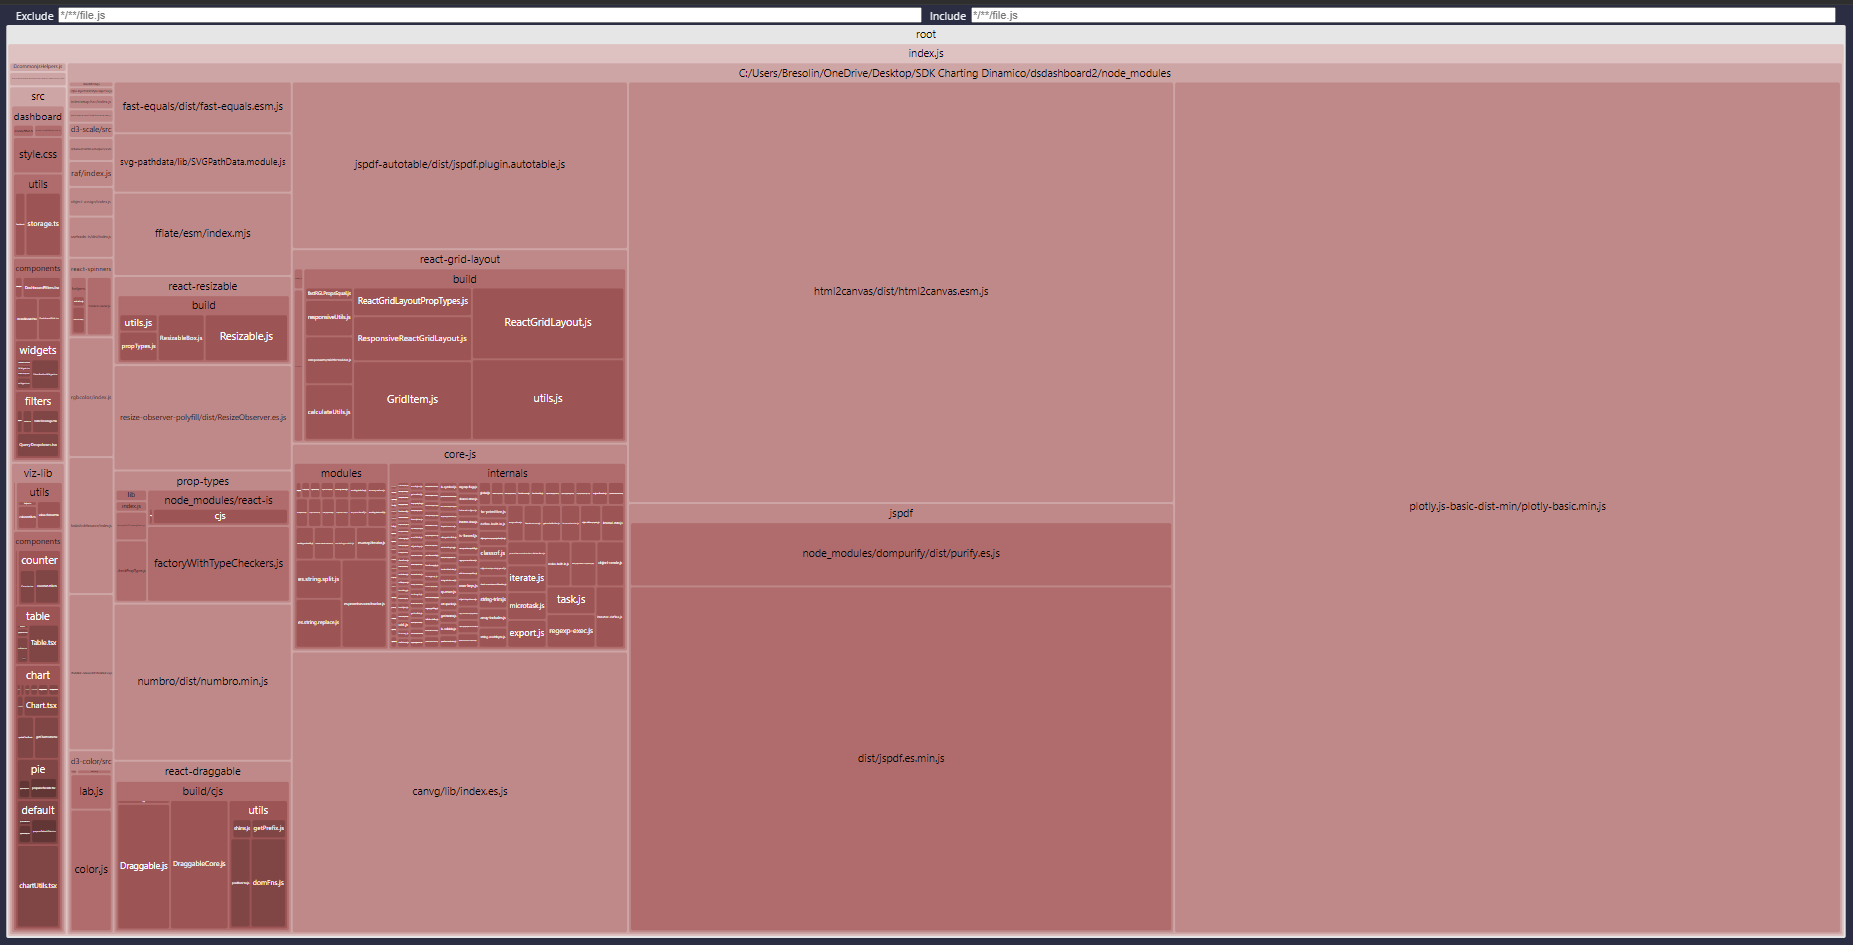
\includegraphics[alt={Esempio di bundle visualizer report}, width=1 \columnwidth]{img/bundle-visualizer.png}
    \caption{Esempio di bundle visualizer report}
    \label{fig:bundle-visualizer}
\end{figure}

\subsection{Componenti}
Nella presente sezione viene descritta l'implementazione delle componenti e delle loro ottimizzazioni all'interno della libreria,
con l'obiettivo di fornire una panoramica sulle funzionalità offerte, sulle tecnologie utilizzate e sul flusso di dati all'interno del sistema.

\subsubsection{Counter}
La componente \textit{Counter} costituisce un contatore che permette di visualizzare un valore numerico all'interno di un widget, associato a un'etichetta
rappresentativa dell'informazione visualizzata. \\
La componente permette inoltre di visualizzare un target, il valore di riferimento da raggiungere, mettendo a disposizione la componente grafica \textit{Knob}
della libreria \textit{PrimeReact} e definendo colori differenti per il valore visualizzato a seconda del raggiungimento o meno del target. \\
La componente offre inoltre la possibilità di visualizzare dei \textit{tooltip}, fornendo informazioni più dettagliate all'utente
in merito ai dati visualizzati, attraverso l'utilizzo dell'attributo \textit{title} associati ai \textit{div} contenenti i valori visualizzati. \\
Le informazioni utilizzare dalla componente vengono elaborata dalla funzione \textit{getCounterData}, chiamata all'interno dell'hook \textit{useMemo}, in modo da
effettuare il ricalcolo dei dati solo in caso di variazione delle props passate alla componente. Questa funzione infatti, a partire dai \textit{data}, dalle \textit{optionsCounter}
(opzioni di visualizzazione ottenute attraverso la concatenzazione delle opzioni di default e le \textit{options} passate come props al componente) e dal \textit{visualizationName}
permette di definite i seguenti valori:
\begin{itemize}
    \item CounterValue: valore numerico del contatore;
    \item TargetValue: valore di riferimento da raggiungere;
    \item CounterLabel: etichetta associata al valore numerico;
    \item CounterValueTooltip: testo del tooltip associato al valore del contatore;
    \item TargetValueTooltip: testo del tooltip associato al valore di riferimento;
    \item TrendPositive: valore booleano che indica se il valore del contatore ha raggiunto o superato il valore target;
    \item ShowTrend: valore booleano che indica se visualizzare o meno il trend del contatore.
\end{itemize}
Le \textit{optionsCounter} definiscono le formattazioni da applicare ai valori calcolati (\ref{counter-format} \textit{Counter: descrizione}), attraverso l'utilizzo della libreria \textit{numbro}. \\
La visualizzazione del trend, determinata dalla variabile \textit{ShowTrend}, viene attivata nel caso vi fosse un target da raggiungere e i valori elaborati
fossero finiti, modificando il colore del valore del contatore e aggiungendo un'icona in base al raggiungimento o meno del valore di riferimento. \\
In merito al rendere la componente responsiva, è stato utilizzato l'hook \textit{useResizeObserver}, fornito dalla libreria \textit{usehook-ts}, per permettere di
aggiornare il fattore di scala per ridimensionare il contenuto in modo che si adatti alle nuove dimensioni del contenitore attraverso la chiamata alla funzione \textit{onScale},
un wrapper di una funzione anonima tramite l'hook \textit{useDebounceCallback} (fornito sempre dalla libreria \textit{usehook-ts}) per evitare chiamate multiple in rapida successione. \\
Tale scala, gestita come stato interno della componente mediante l'hook \textit{useState}, viene passato come parametro alla funzione \textit{getCounterStyles} invocata nella definizione
dello \textit{style} del contenitore dei vari elementi che compongono la componente, la quale ritorna un oggetto di proprietà CSS necessarie per applicare la trasformazione della scala nei
vari browser.

\begin{figure}[H]
    \centering
    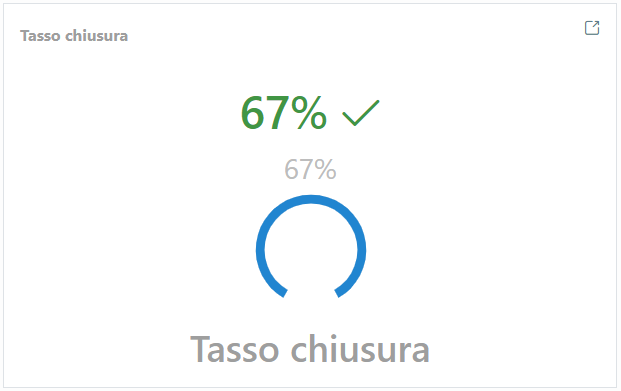
\includegraphics[alt={Esempio di Counter viz-lib con target}, width=0.5 \columnwidth, height=\maxdimen, keepaspectratio]{img/ex_counter.png}
    \caption{Esempio di Counter \textit{viz-lib} con target}
    \label{fig:counter-example}
\end{figure}

\subsubsection{Chart}

\subsubsection{Table}
La componente \textit{Table} costituisce una tabella che permette di visualizzare i dati in forma tabellare. \newline
Tale componente utilizza \textit{DataTable}, una componente resa disponibile dalla libreria \textit{PrimeReact} che offre, attraverso
la definizione di determinate props, di:
\begin{itemize}
    \item alternare i colori delle righe della tabella, al fine di aumentare la leggibilità dei dati visualizzati;
    \item selezionare più righe della tabella, permettendo di effettuare operazioni di \textit{multi-selection} (attraverso
          l'utilizzo di uno \textit{useState});
    \item impostare un filtro globale per la tabella, permettendo di definire su quali colonne effettuare la ricerca dei dati;
    \item impostare un \textit{empty message} personalizzato, visualizzato nel caso in cui la tabella non contenga dati;
    \item ordinare i dati all'interno delle singole colonne, permettendo di visualizzare i dati in ordine crescente o decrescente.
\end{itemize}
Come introdotto nella sezione \ref{item:hookTable}{ \textit{proprietà della componenti: Table}}, la gestione del filtro globale tramite
la funzione \textit{onChangeGlobalFilterValue} presenta l'utilizzo di due valori tramite \textit{useState}:
\begin{itemize}
    \item \textit{globalFilterValueTmp}: stringa utilizzata per memorizzare il valore del filtro impostato all'interno di una
          componente \textit{InputText} di \textit{PrimeReact}, aggiornata in tempo reale all'input fornito dell'utente;
    \item \textit{globalFilterValue}: stringa utilizzata per impostare il valore del filtro globale della tabella, aggiornata
          tramite una chiamata \textit{debounced} di 200 ms alla funzione per settate il valore sullo stato. \newline
          (La funzione \textit{debounced} fa uso dell'hook \textit{useDebounceCallback} fornito dalla libreria \textit{usehook-ts}).
\end{itemize}
Tramite questa implementazione, il recupero dei dati visualizzati all'interno della tabella viene eseguito correttamente, permettendo di risolvere
il bug presente all'interno della componente \textit{DataTable}, il quale comportava la perdita di entry nel caso in cui il filtro globale subisse
più modifiche in rapida successione. \newline
La tabella è resa \textit{scrollable}, impostando una altezza che viene calcolata in modo responsivo a seconda dello spazio disponibile
all'interno del widget in cui è contenuta. \newline
Attraverso la definizione di un \textit{ref} alla componente \textit{DataTable}, è possibile effettuare il download della tabella in formato
\textit{CSV}, tramite l'utilizzo della funzione \textit{exportCSV} resa disponibile dalla libreria \textit{PrimeReact}: tale funzione viene
invocata tramite un \textit{Button} posizionato a fianco della componente \textit{InputText} utilizzata per l'input del filtro globale. \newline
\textbf{Elaborazione dati}\newline
I dati renderizzati all'interno della tabella vengono estratti dal props \textit{data}, passando a sua volta alla componente \textit{DataTable}
tramite la prop \textit{value} l'array \textit{rows} contenente i dati da visualizzare. \newline
Le colonne della tabella sono definite a partire dalle \textit{options} e dai \textit{data} passati come props alla componente \textit{Table}.
Inizialmente sono ridefinite mediante la funzione \textit{getOptions}, la quale imposta delle opzioni di default, ordina la visualizzazione delle colonne
in base all'ordine definito nelle \textit{options}, impostando le proprietà di filtro delle colonne in base alle opzioni indicate e verificando la presenza
di dati all'interno dei \textit{data} (nel caso di assenza di riscontri vengono definite le colonne a partire dai \textit{data}).
Successivamente dalle \textit{options} elaborate vengono definite le vere e proprie colonne della tabella (\textit{tableColumns}), attraverso la funzione \textit{prepareColumns},
la quale attua il filtraggio delle colonne e costruisce l'header delle colonne in base alle opzioni elaborate. \newline
Le \textit{tableColumns} vengono in seguito mappate per creare le componenti \textit{Column} presentate all'interno della tabelle, impostando:
\begin{itemize}
    \item l'header a partire dalle opzioni elaborate;
    \item il \textit{field} a cui fanno riferimento a partire dalle opzioni elaborate;
    \item il props \textit{sortable} per permettere l'ordinamento sulla colonna;
    \item il props \textit{body}, utilizzato per permettere il corretto formattamento e rendering dei dati visualizzati all'interno della singola colonna,
          invocando la funzione \textit{formatRowValue}.
\end{itemize}
Le formattazioni dei dati avvengono mediante i formatter resi disponibili:
\begin{itemize}
    \item \textit{string}: formatta il testo in base indicazioni presenti nell'item, eventualmente restituendo del contenuto HTML;
    \item \textit{datetime}: formatta le date in base alle opzioni elaborate mediante l'uso di \textit{day.js};
    \item \textit{number}: formatta i numeri in base alle opzioni elaborate mediante l'uso di \textit{numbro};
    \item \textit{boolean}: formatta i booleani in base alle opzioni fornite, elaborando anche array;
    \item \textit{json}: formatta i dati JSON in base alle opzioni fornite, permettendo di visualizzare i dati in modo strutturato;
    \item \textit{image}: formatta le immagini in base alle opzioni fornite, permettendo di visualizzare le immagini all'interno della tabella.
\end{itemize}

\begin{figure}[H]
    \centering
    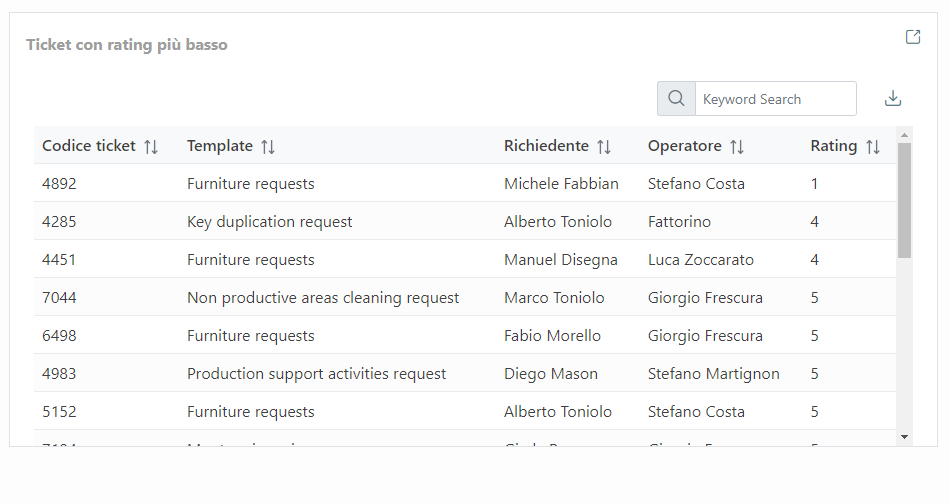
\includegraphics[alt={Esempio di Table viz-lib}, width=1 \columnwidth, height=\maxdimen, keepaspectratio]{img/ex_table.png}
    \caption{Esempio di Table \textit{viz-lib}}
    \label{fig:table-example}
\end{figure}

\subsubsection{Renderer}
La componente \textit{Renderer} costituisce l'entry point della libreria, permettendo di renderizzare tutte le componenti presenti all'interno di
\textit{viz-lib}: per questo motivo tale componente costituisce l'unico \textit{export} della libreria accessibile all'\textit{index.ts} del SDK. \newline
Tale componente costituisce il \textit{wrap} della componente \textit{RendererR}, ottenuto tramite l'utilizzo della funzione \textit{React.memo}.
\begin{adjustwidth}{4em}{0pt}
    \textit{React.memo} è una funzione offerta da \textit{React} per effettuare la \textit{memoization} di una componente funzionale, permettendo di evitare
    nuove renderizzazioni nel caso in cui il componente padre lo richiedesse, a meno che le sue props non abbiano subito modifiche. \newline
    Tale funzione accetta due parametri:
    \begin{itemize}
        \item la componente da memoizzare;
        \item una funzione che accetta due argomenti: le props correnti e le props precedenti della componente, restituendo un valore booleano che indica
              se la componente debba essere renderizzata o meno.
    \end{itemize}
    La presenza del secondo parametro permette di effettuare un controllo specifico, andando a definire i criteri su cui basare i cambiamenti delle props
    rilevanti ai fini della renderizzazione della componente. \newline
\end{adjustwidth}
Nel nostro caso, la funzione \textit{React.memo} utilizza come criterio di controllo tra le props la funzione \textit{isEqual} resa disponibile da \textit{lodash},
la quale permette di effettuare un confronto profondo tra due valori per determinare se sono equivalenti. \newline
\begin{listing}[H]
    \begin{minted}{typescript}
        const Renderer = React.memo(RendererR, (prev, next) =>
            isEqual(prev.data, next.data)
        );
  \end{minted}
    \caption{React.memo della componente Renderer}
    \label{listing:react_memo}
\end{listing}
Per quanto riguarda la componente \textit{RendereR} in questione, essa ricava dai suoi props, tramite l'utilizzo della funzione \textit{getVisualizationType}, il valore
dell'enumerazione \textit{VisualizationType}, assegnandolo alla costante \textit{visualizationType}, in modo da renderizzare la componente corretta in base al tipo di
visualizzazione passato come parametro.

\subsection{Documentazione}
L'implementazione della libreria prodotta è stata documentata tramite l'utilizzo di \textit{Confluence}, la piattaforma
di gestione della conoscenza e di collaborazione sviluppata da \textit{Atlassian}. \newline
La documentazione, su richiesta dell'azienda, è stata redatta in lingua inglese, attraverso una descrizione dettagliata
delle componenti e delle funzionalità offerte dalla libreria. \newline

\begin{figure}[H]
    \centering
    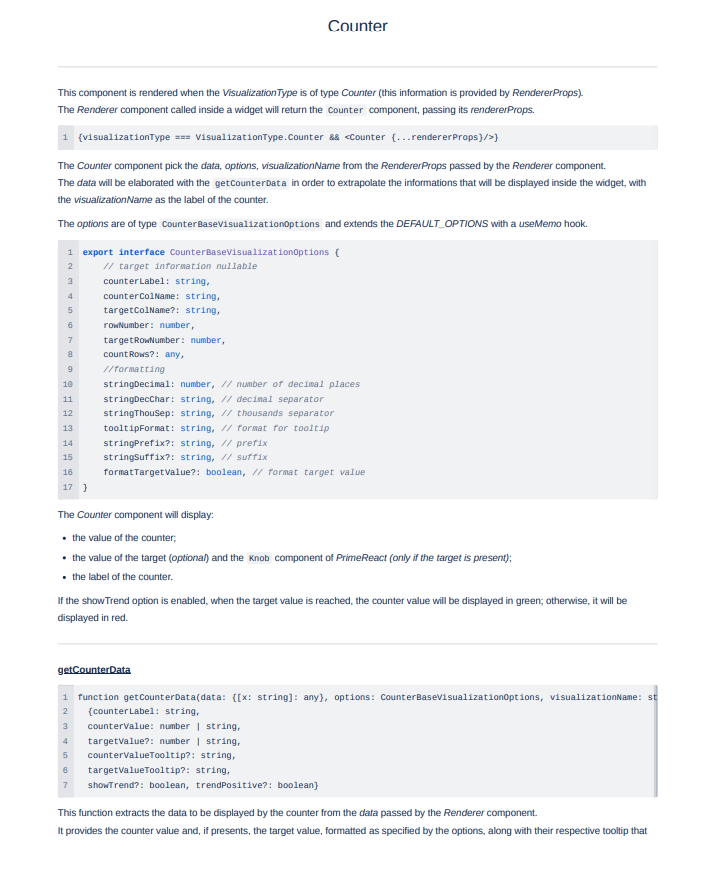
\includegraphics[alt={Esempio documentazione Confluence}, width=1 \textwidth]{img/ex_confluence.png}
    \caption{Esempio documentazione Confluence}
    \label{fig:ex_confluence}
\end{figure}

La documentazione è stata strutturata in modo da essere facilmente consultabile e comprensibile, con l'obiettivo di
fornire un supporto efficace agli sviluppatori futuri che potrebbero dover utilizzare la libreria. \newline
La produzione di una buona documentazione ricopre infatti un ruolo fondamentale al fine di garantire la manutenibilità
del codice e la facilità di comprensione delle funzionalità offerte dalla libreria, in modo da ridurre i tempi di
apprendimento e di sviluppo necessari per gli utilizzi futuri del prodotto implementato.

\section{Testing}
Nella presente sezione verranno descritte le attività di testing effettuate durante lo sviluppo della libreria, con l'obiettivo
di garantire la qualità del prodotto implementato e la corretta esecuzione delle funzionalità offerte.

\subsection{Jest}
Lo strumento utilizzato e configurato all'interno del progetto per l'esecuzione dei test è \textit{Jest}, un framework di testing
per JavaScript sviluppato da \textit{Facebook}. \newline
Jest permette di effettuare test su funzioni, classi e moduli, fornendo un'ampia gamma di funzionalità per la scrittura e l'esecuzione
dei test. \newline
In particolare, Jest offre le seguenti funzionalità:
\begin{itemize}
    \item \textbf{Mocking components}: permette di creare mock di componenti, in modo da simularne il suo comportamento:
          \begin{listing}[H]
              \begin{minted}{typescript}
            jest.mock('percorso.componente', () => ({
                Componente: () => mock_value,
            }));
            \end{minted}
              \caption{Esempio di mock di una componente}
              \label{listing:mock_component}
          \end{listing}
    \item \textbf{Mocking function}: permette di creare mock di funzioni, in modo da simularne il suo comportamento:
          \begin{listing}[H]
              \begin{minted}{typescript}
                jest.spyOn(file_funzione, 'nomeFunzione')
                    .mockReturnValue(mock_value);
            \end{minted}
              \caption{Esempio di mock di una funzione}
              \label{listing:mock_function}
          \end{listing}
    \item \textbf{Suite di test}: permette di creare suite di test, organizzando i test in modo gerarchico:
          \begin{listing}[H]
              \begin{minted}{typescript}
                describe('Nome suite di test', () => {
                    it('Nome test', () => {
                        // Codice del test
                    });
                });
            \end{minted}
              \caption{Esempio di suite di test}
              \label{listing:test_suite}
          \end{listing}
    \item \textbf{Expect}: permette di effettuare asserzioni sui valori restituiti dalle funzioni, verificando la correttezza
          del risultato ottenuto:
          \begin{listing}[H]
              \begin{minted}{typescript}
                    expect(valore).toBe(valore_aspettato);
                \end{minted}
              \caption{Esempio di expect su valore}
              \label{listing:expect}
          \end{listing}
          oppure di verificare la presenza di un elemento all'interno del DOM:
          \begin{listing}[H]
              \begin{minted}{typescript}
                    expect(screen.getByText('Testo')).toBeInTheDocument();
                \end{minted}
              \caption{Esempio di expect su elemento del DOM}
              \label{listing:expect_dom}
          \end{listing}
\end{itemize}
La sua configurazione è stata effettuata all'interno del file \textit{packages.json}, in cui sono state definite le impostazioni di
esecuzione dei test e le dipendenze necessarie per il loro corretto funzionamento, come il preset che consente di utilizzare \textit{Typescript},
l'ambiente di test \textit{jsdom} che simula un ambiente browser e i vari formati di file che deve considerare o ignorare. \newline
Di seguito viene riportata la configurazione utilizzata.
\begin{listing}[H]
    \begin{minted}{json}
    "jest": {
        "preset": "ts-jest",
        "testEnvironment": "jsdom",
        "moduleFileExtensions": [
            "ts",
            "tsx",
            "js",
            "jsx",
            "json",
            "node"
        ],
        "transform": {
            "^.+\\.(ts|tsx)$": "ts-jest",
            "^.+\\.(js|jsx)$": "babel-jest"
        },
        "transformIgnorePatterns": [
            "node_modules/(?!(d3-color)/)"
        ]
    }
    \end{minted}
    \caption{Configurazione Jest all'interno del file packages.json}
    \label{listing:jest_config}
\end{listing}

\subsection{Unit testing}
Per garantire la correttezza delle funzionalità offerte dalla libreria, è stato effettuato un processo di testing a livello di unità. \newline
Nel presente progetto sono stati implementati test per le singole componenti, mockando le dipendenze esterne ed eventuali altre componenti
della libreria utilizzate, verificando il corretto funzionamento all'interno della singola unità.

\begin{listing}[H]
    \begin{minted}[escapeinside=||]{typescript}
    jest.mock('./charts/Counter', () => ({
        Counter: () => <div>Counter Component|</|div>,
    }));

    jest.mock('./charts/Chart', () => ({
        Chart: () => <div>Chart Component|</|div>,
    }));

    jest.mock('./charts/Table', () => ({
        Table: () => <div>Table Component|</|div>,
    }));

    describe('Renderer test right components', () => {
        it('renders Counter component when visualizationType is Counter', 
            () => {
            jest.spyOn(helper, 'getVisualizationType')
                .mockReturnValue(VisualizationType.Counter);

            const rendererProps: RendererProps = {
                visualizationName: 'Counter',
                type: 'Counter',
                data: {},
                options: {},
            };

            render(<Renderer {...rendererProps} />);

            expect(screen.getByText('Counter Component')).toBeInTheDocument();
            });
    // ...
    });
    \end{minted}
    \caption{Esempio di unit test: Renderer component}
    \label{listing:test_Renderer}
\end{listing}

Come si può osservare nell'esempio di codice riportato in \ref{listing:test_Renderer}, è stato effettuato un test sulla componente \textit{Renderer},
mockando le componenti \textit{Counter}, \textit{Chart} e \textit{Table} utilizzate all'interno della componente stessa, verficando che venga renderizzata
la componente corretta in base al tipo di visualizzazione passato come parametro. \newline
Il tipo di visualizzazione a sua volta viene ottenuto dal mock della funzione \textit{getVisualizationType}, la quale restituisce il tipo di visualizzazione
corretto in base al parametro passato come props al Renderer: in questo modo viene garantita la corretta logica della singola componente, senza far affidamento
su funzioni o componenti esterne. \newline
La correttezza delle funzioni è stata verificata tramite appositi test di unità sulle singole funzioni, eventualmente mockando le dipendenze esterne utilizzate
all'interno della funzione stessa, in modo da garantire la correttezza logica implementata. \newline
Di seguito viene riportato un esempio di test di unità effettuato sulla funzione \textit{getVisualizationType}.

\begin{listing}[H]
    \begin{minted}{typescript}
    it('should return VisualizationType.Table when type is TABLE', () => {
        expect(
            getVisualizationType('TABLE')
        ).toBe(VisualizationType.Table);
    });
    \end{minted}
    \caption{Esempio di unit test: getVisualizationType}
    \label{listing:test_getVisualizationType}
\end{listing}

\subsection{Integration testing}
Per garantire la corretta integrazione delle componenti all'interno della libreria, è stato effettuato un processo di testing a livello di integrazione,
tramite l'utilizzo di \textit{Jest}. \newline
I test di integrazione permettono di verificare il corretto funzionamento delle componenti all'interno del sistema, testando il comportamento
dei singoli moduli all'interno del contesto in cui sono utilizzati. \newline
Nel presente progetto sono stati implementati test di integrazione per verificare il corretto funzionamento delle componenti in relazione con dipendenze
esterne.

\begin{listing}[H]
    \begin{minted}[escapeinside=||]{typescript}
    jest.mock('./charts/Counter', () => ({
        Counter: () => <div>Counter Component|</|div>,
    }));

    jest.mock('./charts/Chart', () => ({
        Chart: () => <div>Chart Component|</|div>,
    }));

    jest.mock('./charts/Table', () => ({
        Table: () => <div>Table Component|</|div>,
    }));
    
    describe('Renderer test right components', () => {
        it('renders Counter component when visualizationType is Counter', () => {

            const rendererProps: RendererProps = {
                visualizationName: 'Counter',
                type: 'Counter',
                data: {},
                options: {},
            };

            render(<Renderer {...rendererProps} />);

            expect(screen.getByText('Counter Component')).toBeInTheDocument();
        });
    // ...
    });
    \end{minted}
    \caption{Esempio di integration test: Renderer component}
    \label{listing:test_Renderer_integration}
\end{listing}

Come si può osservare nell'esempio di codice riportato in \ref{listing:test_Renderer_integration}, è stato effettuato un test di integrazione sulla componente \textit{Renderer},
mockando le componenti \textit{Counter}, \textit{Chart} e \textit{Table} utilizzate all'interno della componente stessa, verficando che venga renderizzata
la componente corretta in base al tipo di visualizzazione passato come parametro. \newline
Il tipo di visualizzazione a sua volta viene ottenuto internamente alla componente grazie alla funzione \textit{getVisualizationType}, la quale restituisce il tipo di visualizzazione
corretto in base al parametro passato come props al Renderer: in questo modo viene garantita la corretta integrazione delle componenti all'interno del sistema, testando il comportamento
delle unità in relazione tra loro all'interno del contesto in cui sono utilizzate.